% |R(mu)|^2 = h0^2/(mu - 6)^2 + h3^2/(mu + 4)^2 with h0 = h3 = sqrt 2 (prior at 90 degrees, beta = 2)
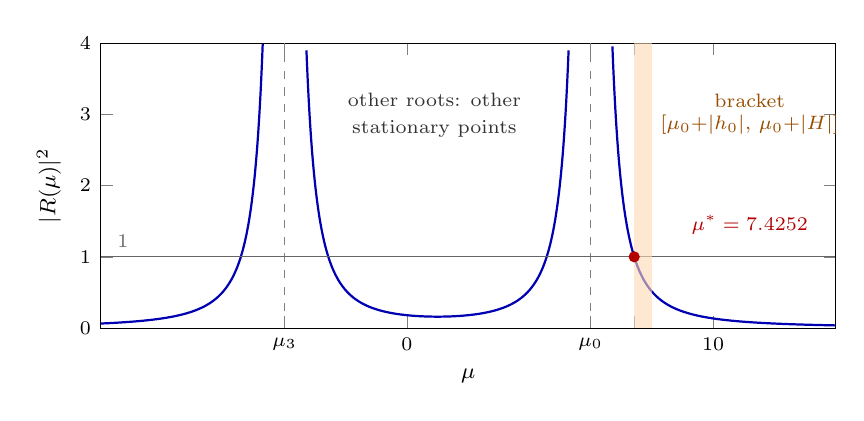
\begin{tikzpicture}
  \begin{axis}[width=0.9\textwidth, height=5.2cm, xmin=-10, xmax=14, ymin=0, ymax=4, restrict y to domain=0:4,
      xlabel={$\mu$}, ylabel={$|R(\mu)|^2$}, xtick={-4,0,6,7.4142,10}, xticklabels={$\mu_3$,$0$,$\mu_0$,,$10$},
      tick label style={font=\scriptsize}, label style={font=\footnotesize}, samples=600, unbounded coords=jump]
    \addplot[thick, blue!70!black, domain=-10:-4.02] {2/(x-6)^2 + 2/(x+4)^2};
    \addplot[thick, blue!70!black, domain=-3.98:5.98] {2/(x-6)^2 + 2/(x+4)^2};
    \addplot[thick, blue!70!black, domain=6.02:14] {2/(x-6)^2 + 2/(x+4)^2};
    \draw[gray, dashed] (axis cs:-4,0) -- (axis cs:-4,4);
    \draw[gray, dashed] (axis cs:6,0) -- (axis cs:6,4);
    \draw[black!60] (axis cs:-10,1) -- (axis cs:14,1) node[pos=0.03, above, font=\scriptsize] {$1$};
    \fill[orange!30, opacity=0.6] (axis cs:7.4142,0) rectangle (axis cs:8,4);
    \addplot[only marks, mark=*, mark size=1.8pt, red!70!black] coordinates {(7.42517,1)};
    \node[font=\scriptsize, red!70!black] at (axis cs:11.2,1.45) {$\mu^* = 7.4252$};
    \node[font=\scriptsize, orange!60!black, align=center] at (axis cs:11.2,3.0) {bracket\\ $[\mu_0 {+} |h_0|,\, \mu_0 {+} |H|]$};
    \node[font=\scriptsize, gray!40!black] at (axis cs:0.9,3.2) {other roots: other};
    \node[font=\scriptsize, gray!40!black] at (axis cs:0.9,2.8) {stationary points};
  \end{axis}
\end{tikzpicture}
